% \section*{Vtx distributions}
% \begin{figure}
%     \centering
%     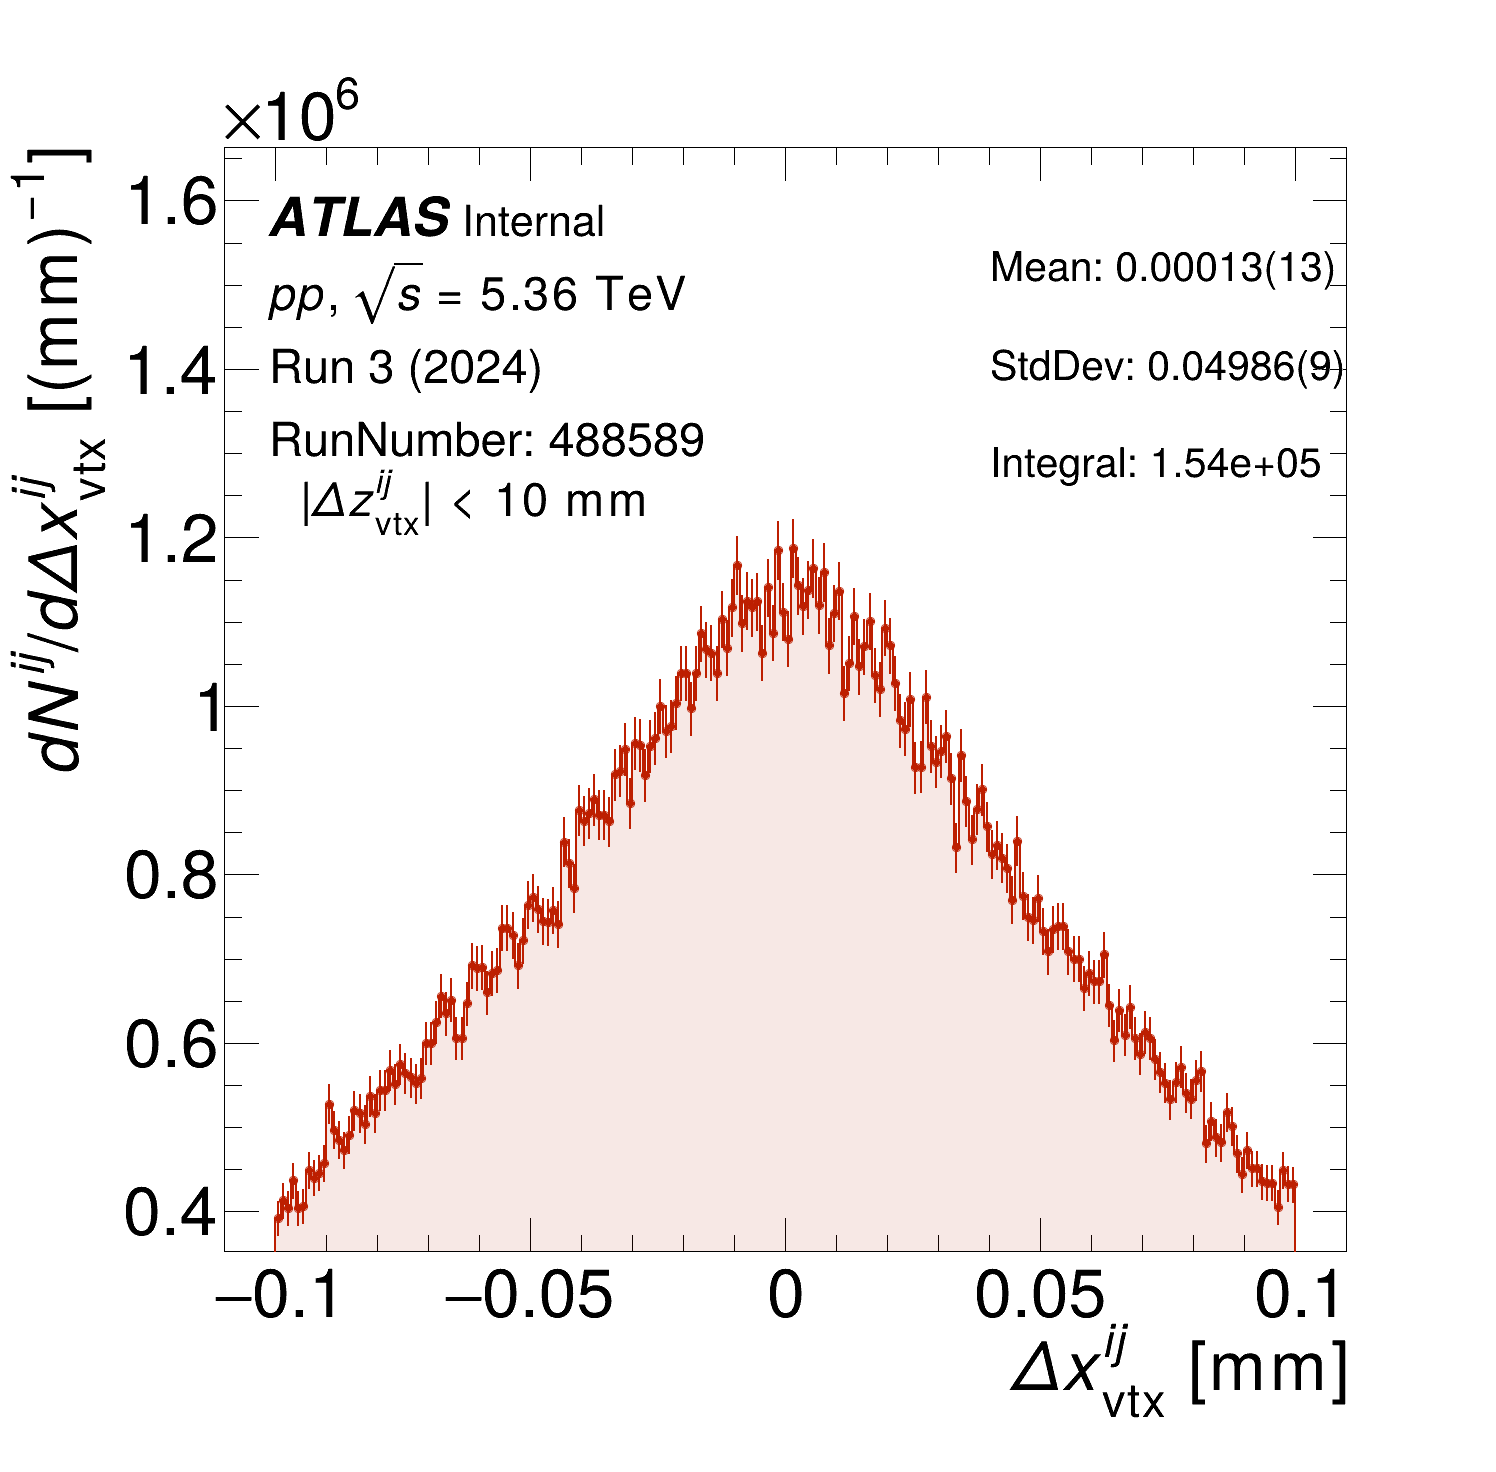
\includegraphics[width=0.48\linewidth]{images/vertex_x_dist_488589.png}
%     \hskip10pt
%     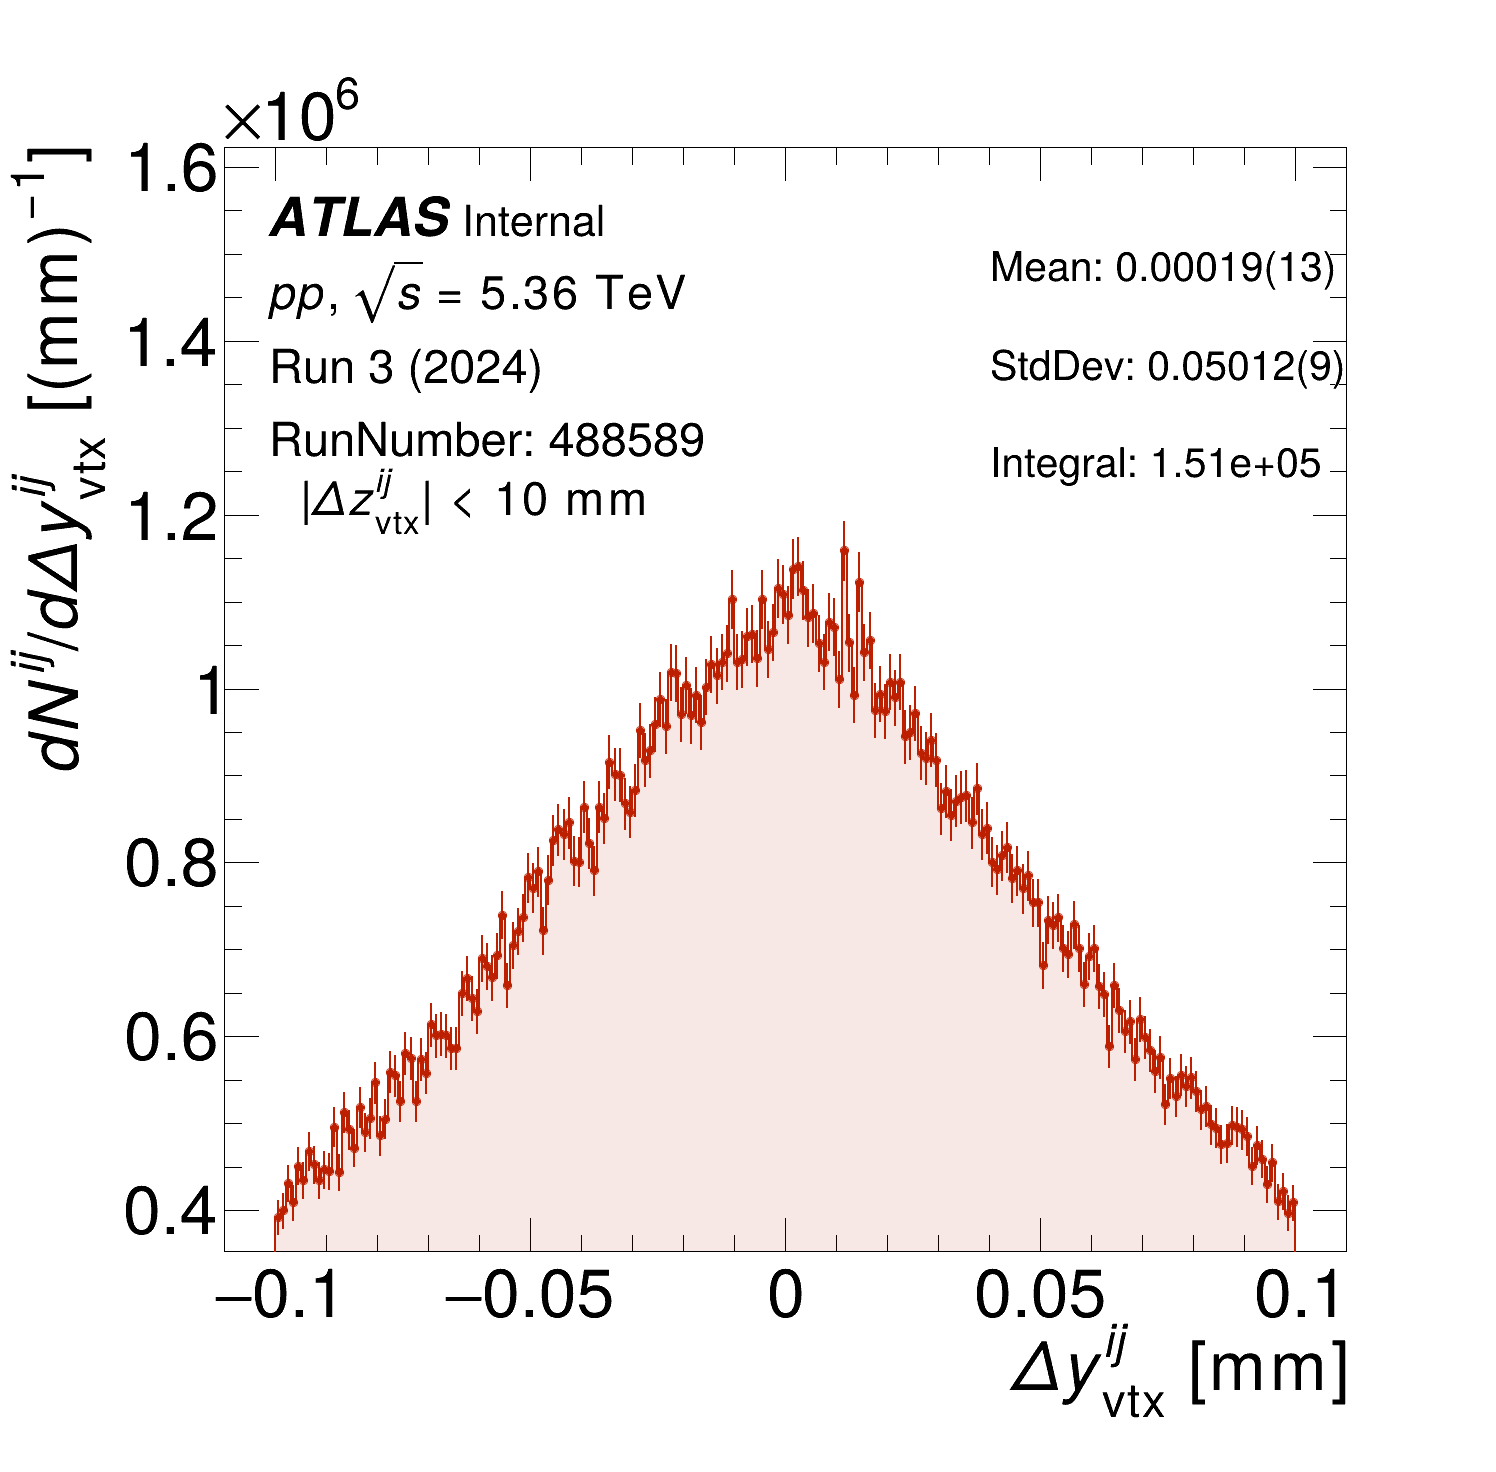
\includegraphics[width=0.48\linewidth]{images/vertex_y_dist_488589.png}
%     \caption{Distributions of pair-wise distances of vertices in $x$ and $y$ coordinates within the ''dip'' region of $\Delta z$ < \qty{10}{\mm}}
%     \label{fig:app_vtx_xy}
% \end{figure}

\begin{figure}[h]
    \centering
    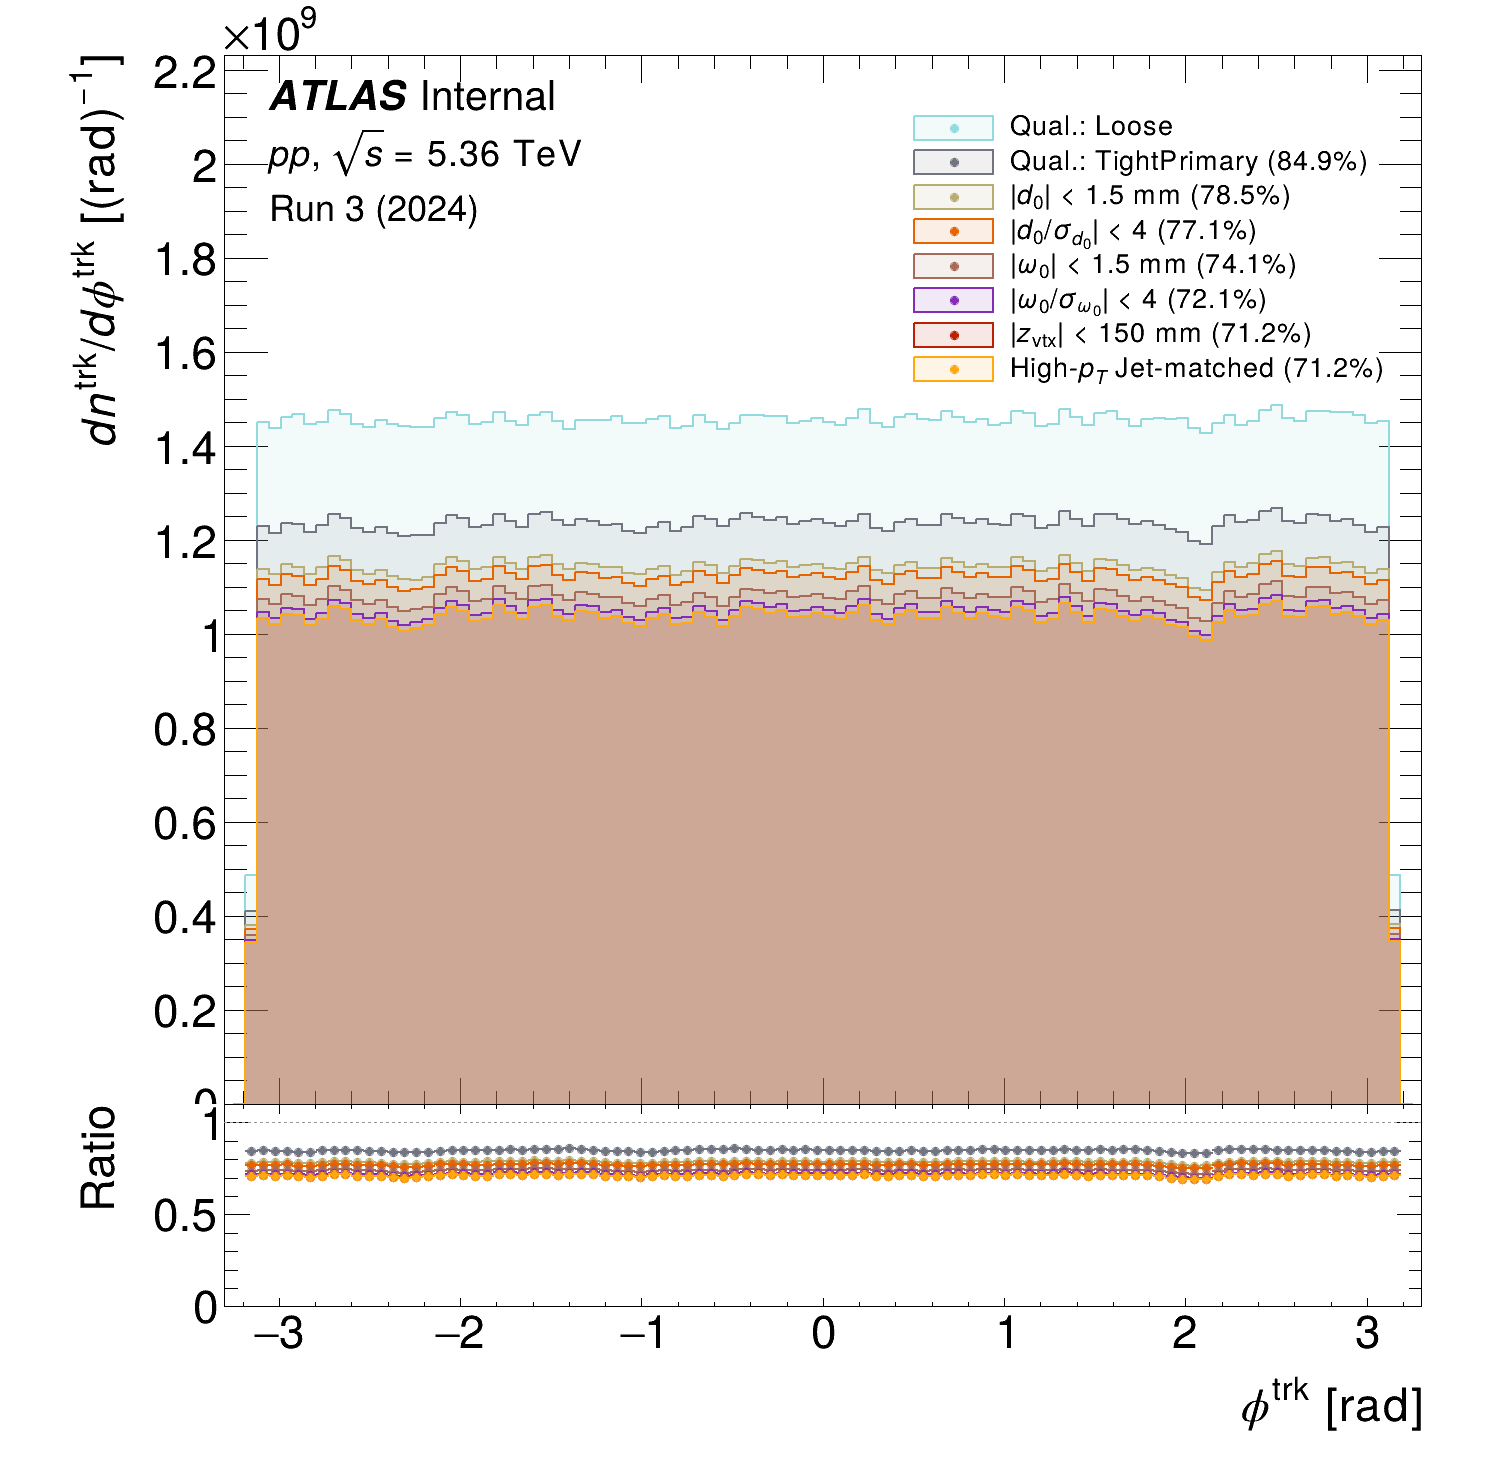
\includegraphics[width=0.49\linewidth]{images/trk_phi_cutflow_.png}
    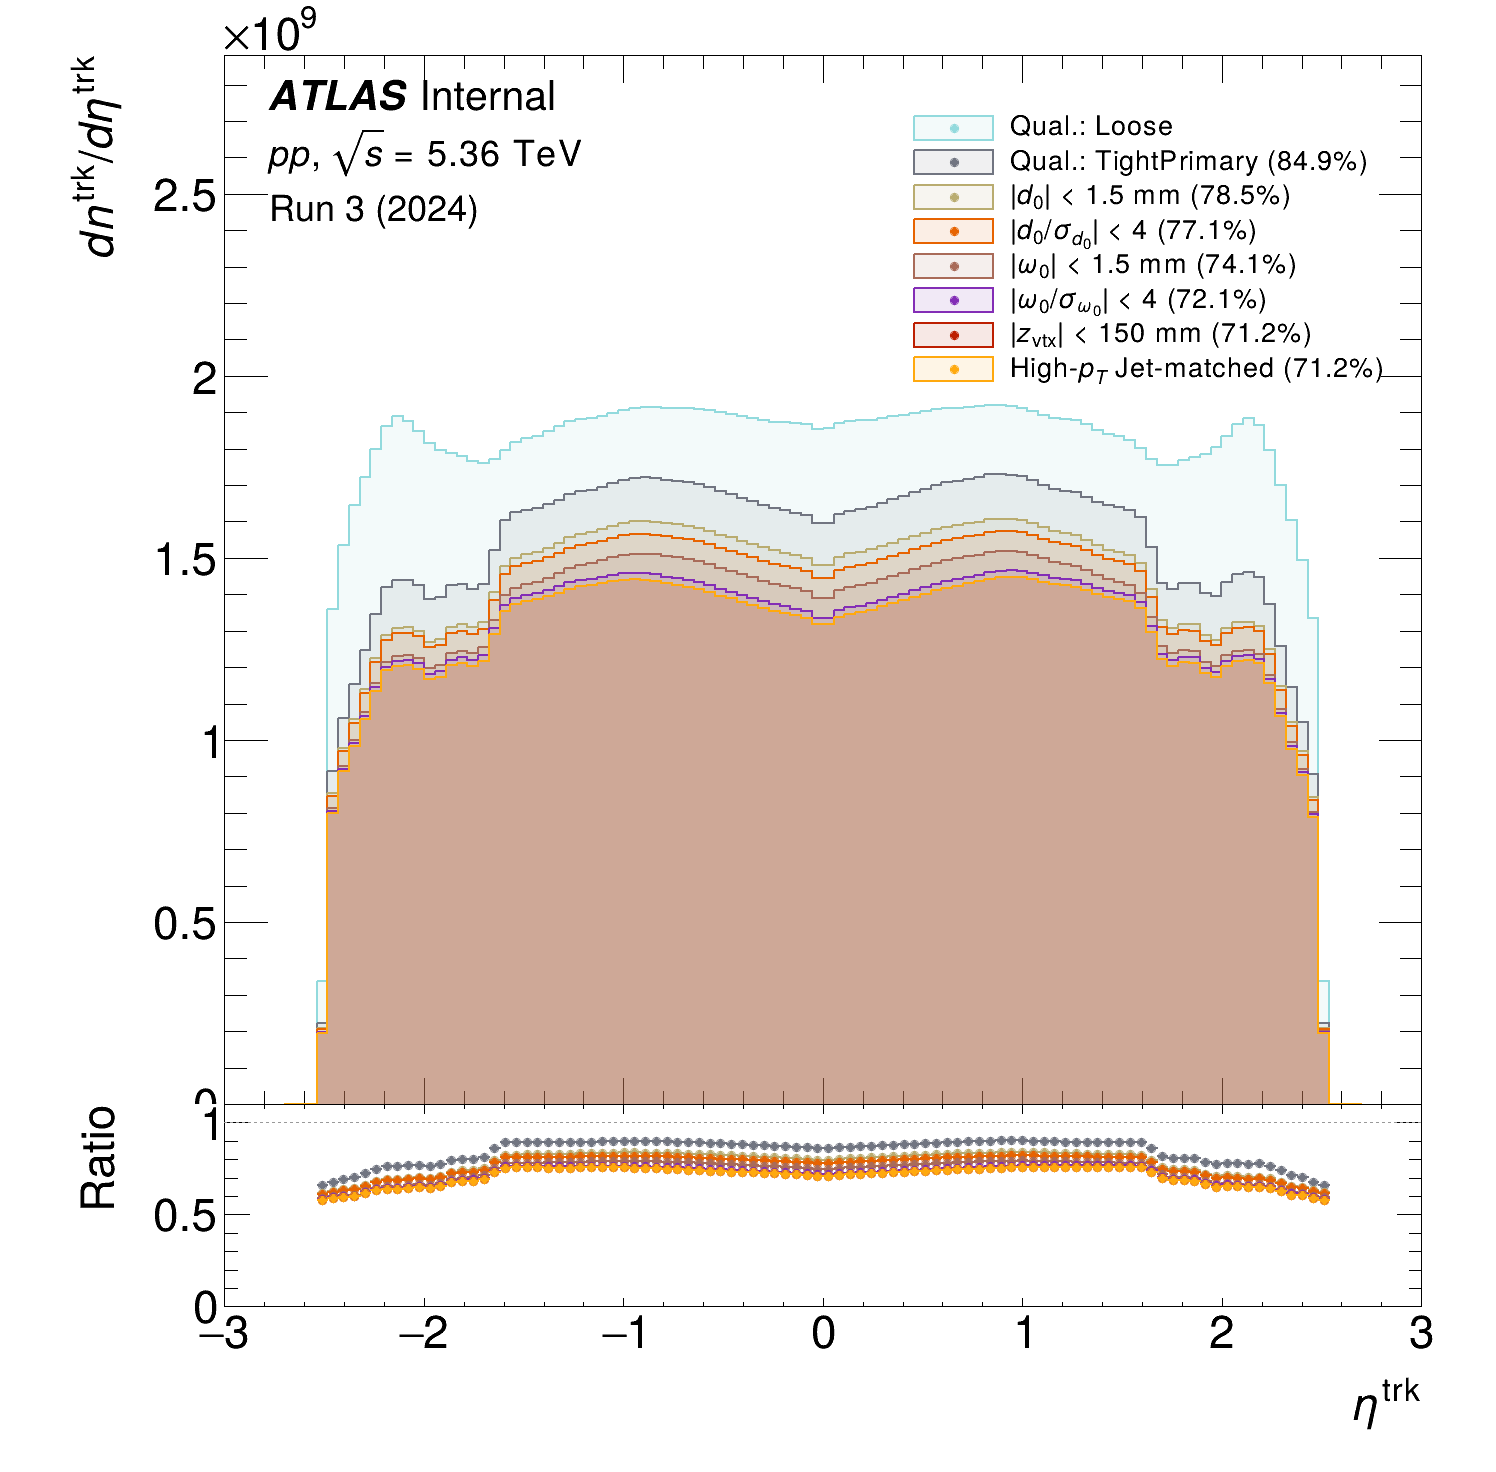
\includegraphics[width=0.49\linewidth]{images/trk_eta_cutflow_.png}
    \caption{Cutflows of $\eta$ and $\phi$ distributions in $\pprefSample$}
    \label{fig:cutflow_eta_phi}
\end{figure}

\begin{figure}[h]
    \centering
    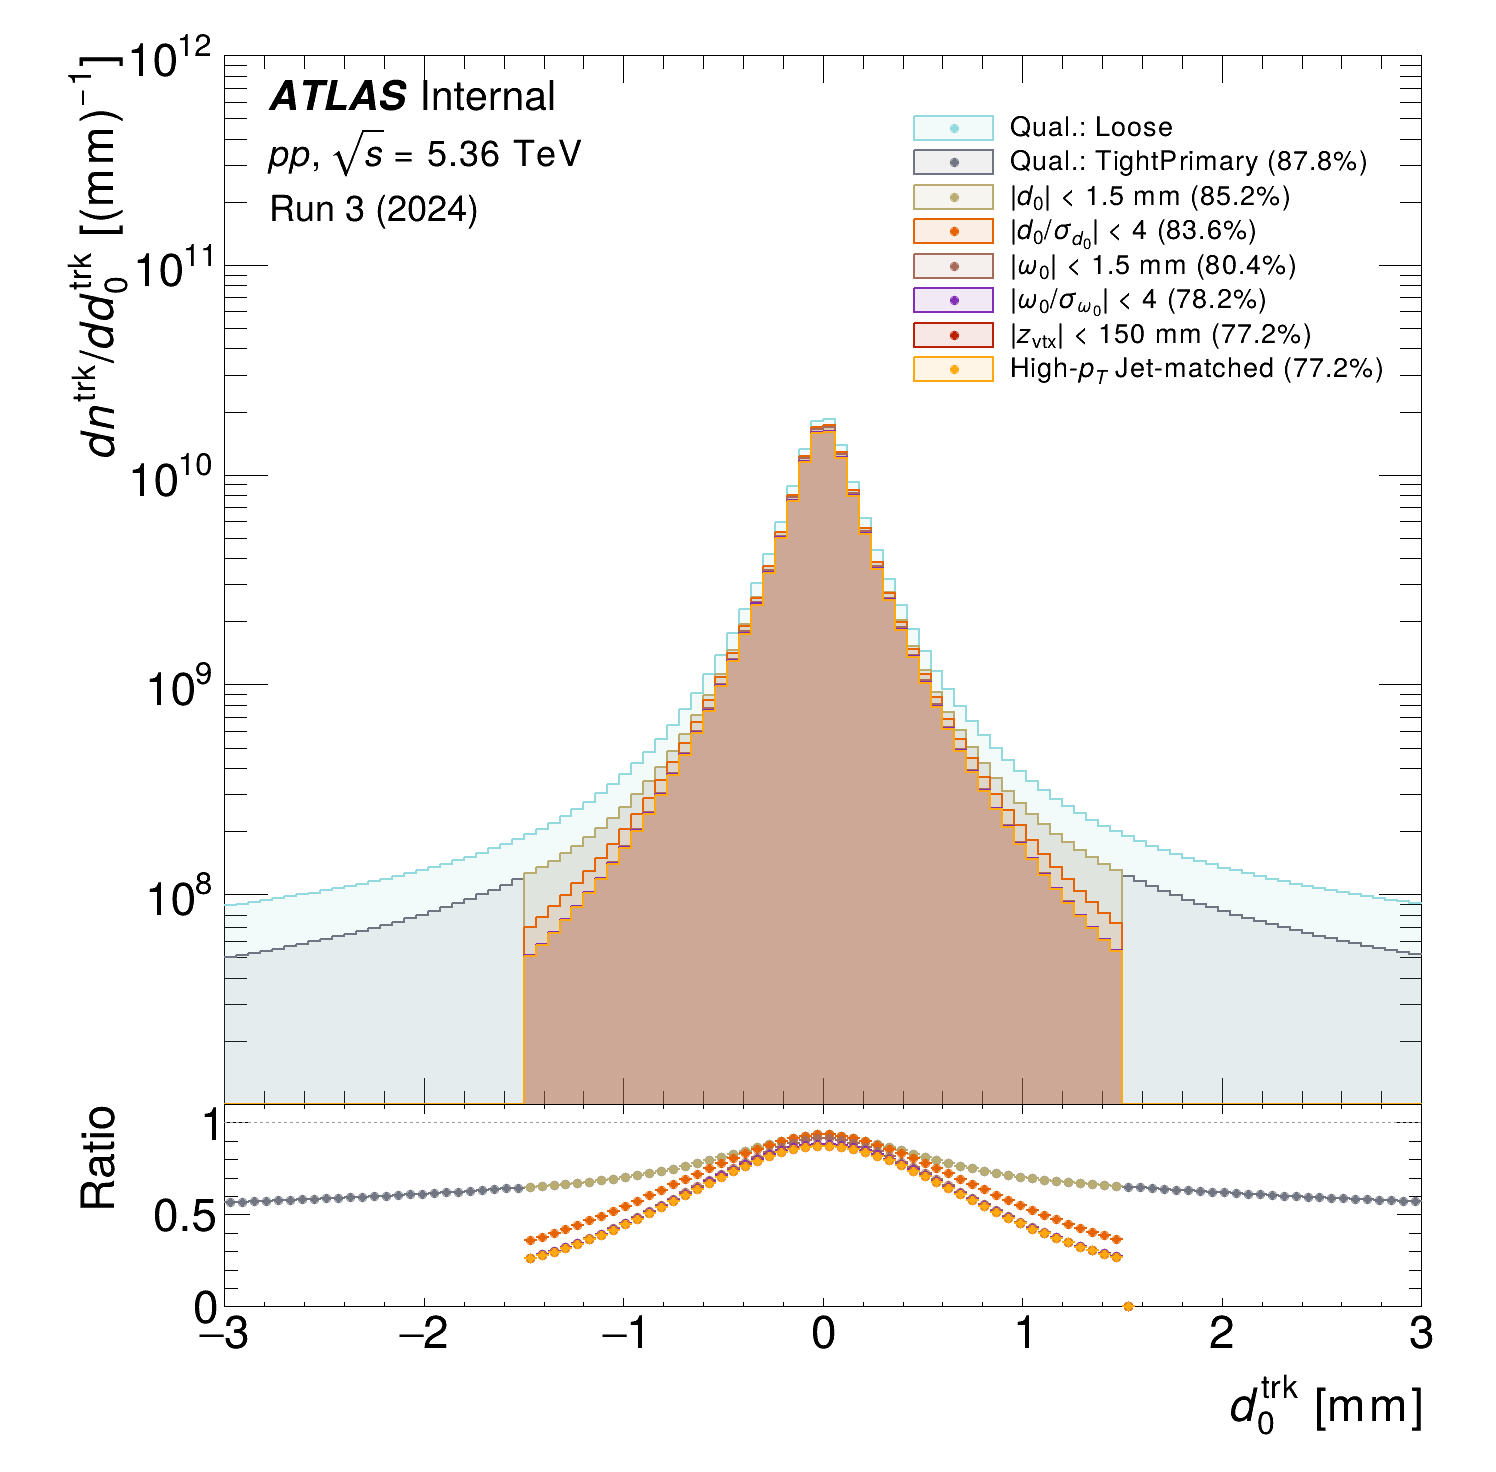
\includegraphics[width=0.49\linewidth]{images/trk_d0_cutflow_.png}
    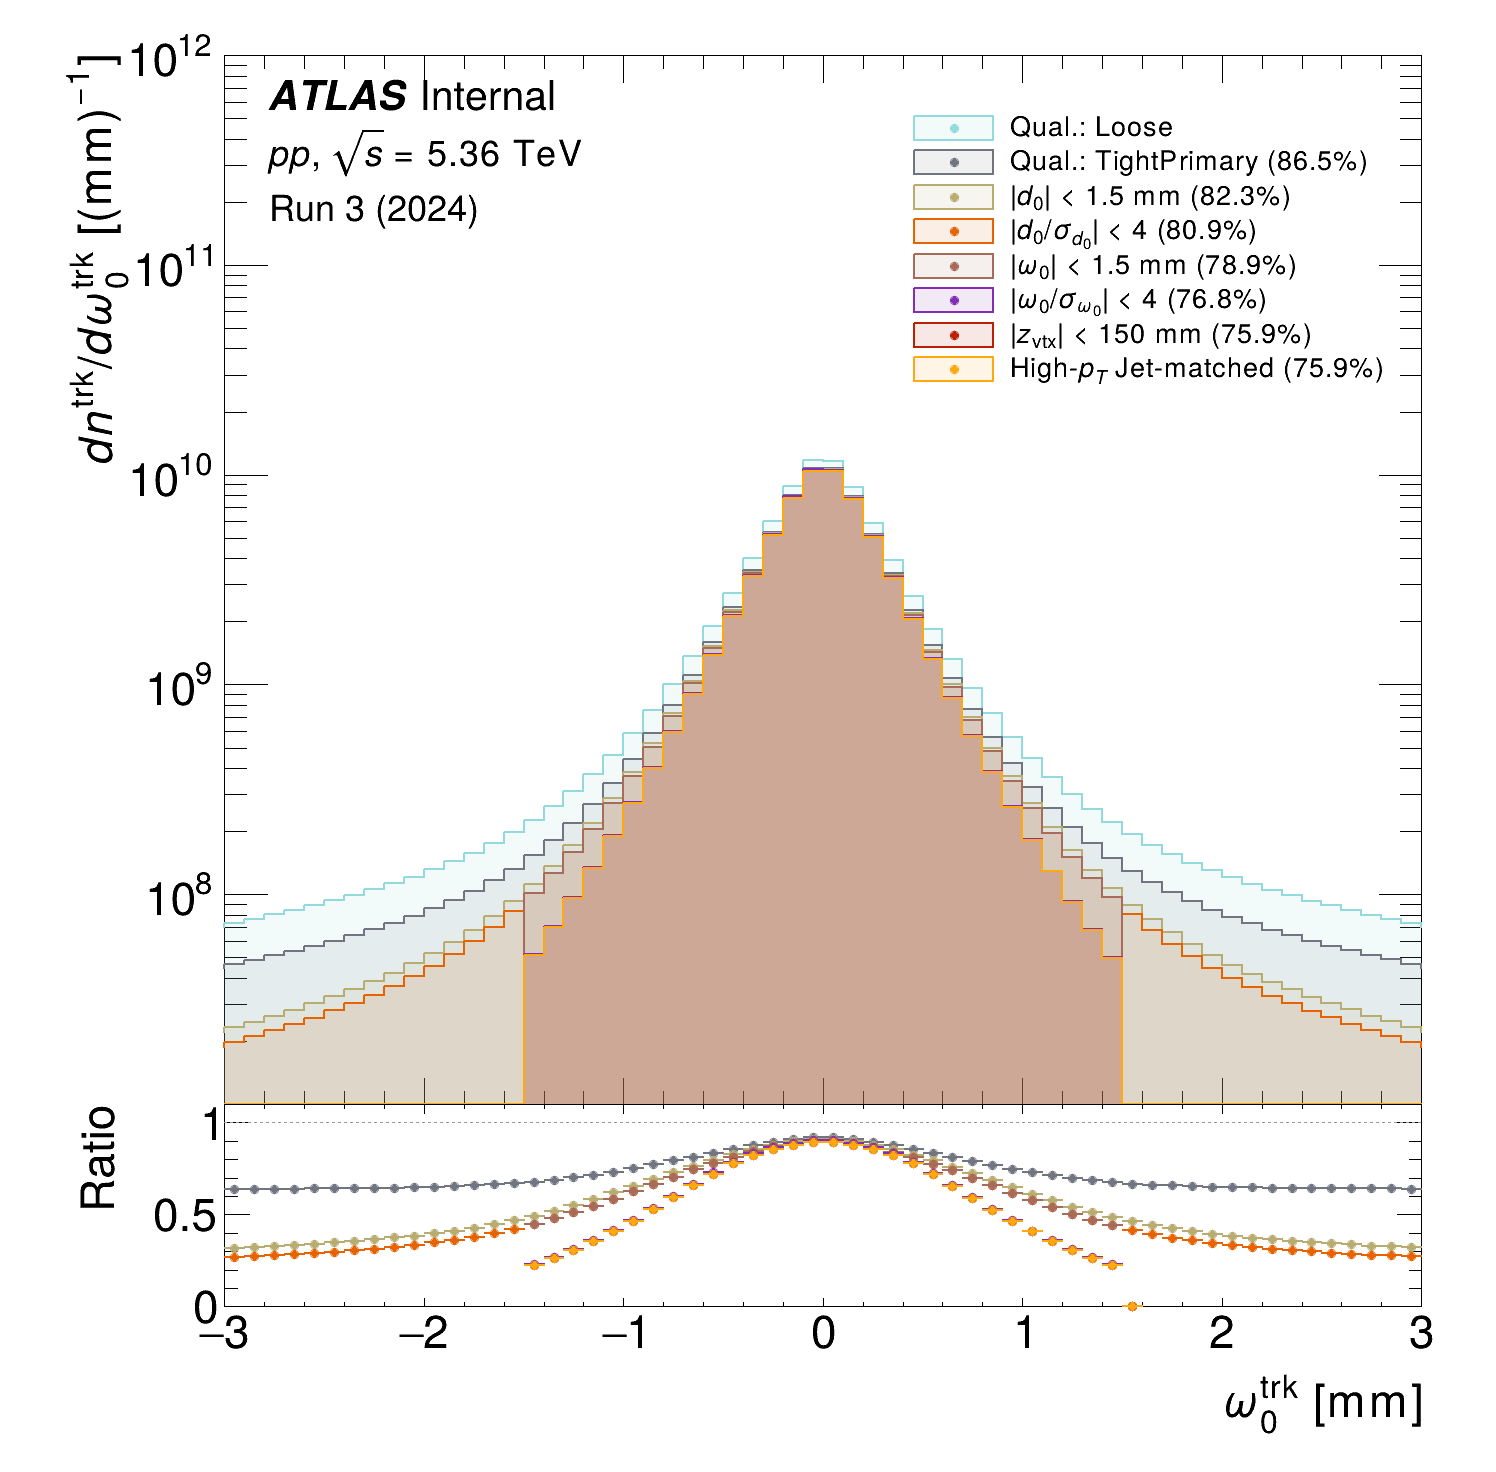
\includegraphics[width=0.49\linewidth]{images/trk_omega0_cutflow_.png}
    \caption{Cutflows of $d_0$ and $\omega_0$ distributions in $\pprefSample$}
    \label{fig:cutflow_d0_omega0}
\end{figure}

\begin{figure}[h]
    \centering
    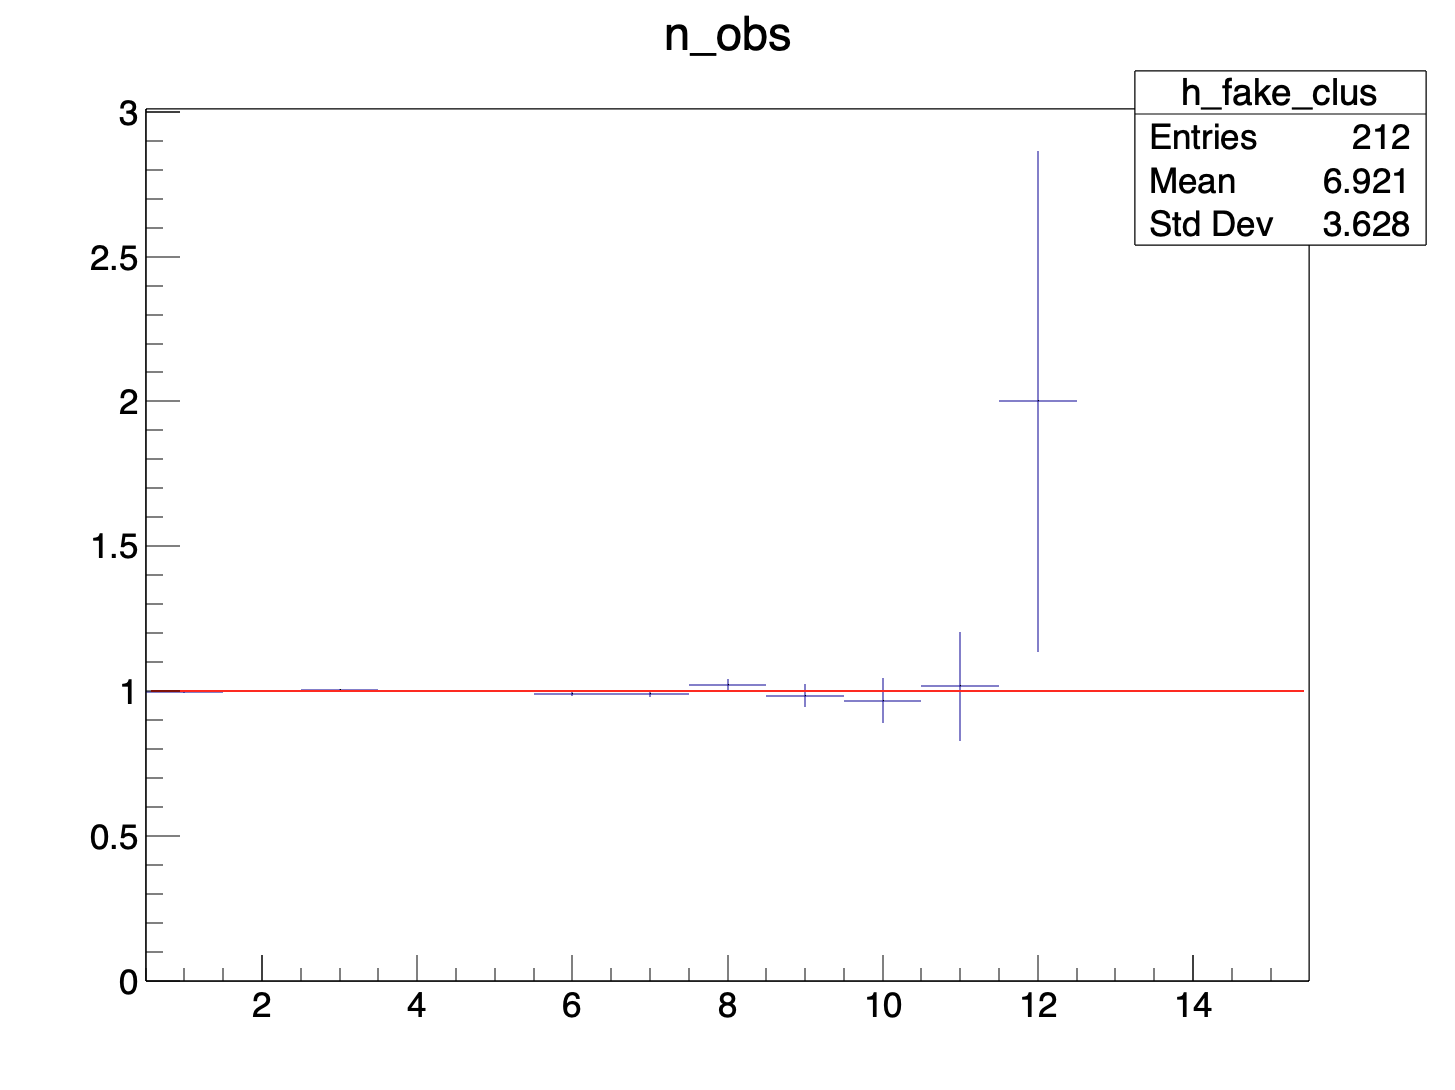
\includegraphics[width=0.5\linewidth]{images/comp_clus_seq_merger.png}
    \caption{Ratio of observed distributions $N_\text{gen}^\text{obs}$ of number of vertices after merging for two algorithms (sequential and clustered). The ratio is consistent with 1 for fit with $\chi^2/\text{ndf}=7.5/11$ and $\text{const}=0.999 \pm0.001$}
    \label{fig:ratio_seq_clus_merger}
\end{figure}